\documentclass[a4paper,twoside,12pt]{book}


\usepackage[italian]{babel}
\usepackage[latin1]{inputenc}
\usepackage[dvips]{epsfig}
\DeclareGraphicsExtensions{.ps,.eps}
\usepackage{subfigure}
\usepackage[T1]{fontenc}

\usepackage{fancyhdr}
\usepackage{amsmath}
\usepackage{amssymb}
\usepackage{a4}
\newcommand{\clearemptydoublepage}{\newpage{\pagestyle{empty}\cleardoublepage}}
\newcommand{\nohyphens}{\hyphenpenalty=10000\exhyphenpenalty=10000\relax}

%% Layout della pagina
%\pagestyle{fancyplain}
%\setlength{\headheight}{14.5pt}
%\addtolength{\headwidth}{\marginparsep}
%\addtolength{\headwidth}{\marginparwidth}
%\renewcommand{\chaptermark}[1]{\markboth{#1}{}}
%\renewcommand{\sectionmark}[1]{\markright{\thesection\  #1}}
%\lhead[\fancyplain{}{\bfseries\thepage}]%
%      {\fancyplain{}{\bfseries\rightmark}}
%\rhead[\fancyplain{}{\bfseries\leftmark}]%
%      {\fancyplain{}{\bfseries\thepage}}
%\cfoot{}

% Questa lunghezza rappresenta la lunghezza completa della pagine, compreso
% lo spazio per le note a margine
%\newlength{\fullpagelen}
%\setlength{\fullpagelen}{\textwidth}
%\addtolength{\fullpagelen}{\marginparsep}
%\addtolength{\fullpagelen}{\marginparwidth}

\makeatletter
\renewenvironment{thebibliography}[1]
  {%
    \chapter*{\bibname}%
    \addcontentsline{toc}{chapter}{\bibname}%
    \@mkboth{\MakeUppercase\bibname}{\MakeUppercase\bibname}%
    \list{\@biblabel{\@arabic\c@enumiv}}%
    {%
      \settowidth\labelwidth{\@biblabel{#1}}%
      \leftmargin\labelwidth
      \advance\leftmargin\labelsep
      \@openbib@code
      \usecounter{enumiv}%
      \let\p@enumiv\@empty
      \renewcommand\theenumiv{\@arabic\c@enumiv}%
    }%
    \sloppy
    \clubpenalty4000
    \@clubpenalty \clubpenalty
    \widowpenalty4000%
    \sfcode`\.\@m%
  }%
  {%
    \def\@noitemerr
    {\@latex@warning{Empty `thebibliography' environment}}%
    \endlist%
  }   % Finisce qui la ridefinizione di thebibliography

\makeatother



\begin{document}


\pagestyle{fancy}
\renewcommand{\chaptermark}[1]{\markboth{#1}{}}
\renewcommand{\sectionmark}[1]{\markright{\thesection\ #1}}
\fancyhf{} \fancyhead[LE,RO]{\bfseries\thepage}
\fancyhead[LO]{\bfseries\rightmark}
\fancyhead[RE]{\bfseries\leftmark}
\renewcommand{\headrulewidth}{0.5pt}
\renewcommand{\footrulewidth}{0pt}
 \fancypagestyle{plain}{
\fancyhead{}
\renewcommand{\headrulewidth}{0pt}}


\thispagestyle{empty} \vspace*{\stretch{1}} \hfill\begin{minipage}[t]{.618\linewidth}
\flushright\itshape Dedicata a chi vi pare :-) .
\end{minipage}
\vspace*{\stretch{3}}
 \clearemptydoublepage
\chapter*{{\em Ringraziamenti}}

\emph{ Ringraziate chi vi pare...}
\clearemptydoublepage
\thispagestyle{empty}
\chapter*{Prefazione}

Blablabla
\clearemptydoublepage
\tableofcontents \clearemptydoublepage

\chapter{Introduzione}


\section{Stream Processing}
\section{Semantic Web}
\section{Stream Reasoning}
\subsection{RDF Stream Processing}
\subsection{RSP Engine - Existing Solutions}

\section{Contributions}
\subsection{Heaven}
\subsection{RSPEngine inside DSMS}
\subsection{Experiments}

\section{Structure of this Thesis}

Blablabla

Esempio di figura

\begin{figure}[ht]
\centerline{\epsfig{file=esempio.ps, width=12 true cm}}
\caption{Didascalia esempio di figura.}
\label{fig:esempio}
\end{figure}

Esempio di equazione

\begin{equation}
\dot V_4= - k_v \lambda (z_1- \varepsilon \lambda z_3)^T(z_1-
\varepsilon \lambda z_3).
\end{equation}
 \clearemptydoublepage
\chapter{Heaven}

\section{Requirements}


\section{Architecture}
\subsection{Streamer}
\subsection{Result Collector}
\subsection{RSP Engine}
\subsection{Test Stand}
\subsection{Analyser}
\section{Implementation}
\subsection{Streamer - RDF2RDFStream}
\subsection{Result Collector}
\subsection{RSP Engine - Esper Integration}
\subsection{Test Stand}
\subsection{Analyser}

\section{Baselines}
\subsection{Time Control}
\subsection{Stream Model}
\subsection{Reasoning}


Esempio di figura

\begin{figure}[ht]
\centerline{\epsfig{file=esempio.ps, width=12 true cm}}
\caption{Didascalia esempio di figura.}
\label{fig:esempio}
\end{figure}

Esempio di equazione

\begin{equation}
\dot V_4= - k_v \lambda (z_1- \varepsilon \lambda z_3)^T(z_1-
\varepsilon \lambda z_3).
\end{equation}
 \clearemptydoublepage
\chapter{RSPEngine}


\section{Architectural Variants}
\subsection{Plain}
\subsection{CEP on RDF}
\subsection{CEP on Ontology RDF Stream}

Blablabla

Esempio di figura

\begin{figure}[ht]
\centerline{\epsfig{file=esempio.ps, width=12 true cm}}
\caption{Didascalia esempio di figura.}
\label{fig:esempio}
\end{figure}

Esempio di equazione

\begin{equation}
\dot V_4= - k_v \lambda (z_1- \varepsilon \lambda z_3)^T(z_1-
\varepsilon \lambda z_3).
\end{equation}
 \clearemptydoublepage
\chapter{Experiments}

\section{Experimental Model} 
%Ognuno viene eseguito nelle varianti, Graph, Stmt, RHODF, SMPL, INC, Naive, Tempo Controllato esternamente e non. 
\subsection{SOAK}
\subsection{Step Linear Response}
\subsection{Step Degree of Magnitude Response}

\section{Experimental Results}

\subsection{SOAK}
\subsection{Step Linear Response}
\subsection{Step Degree of Magnitude Response} \clearemptydoublepage

\include{AppendiceA} \clearemptydoublepage

\nocite{*}
\bibliographystyle{plain}
\bibliography{thesis}


\clearemptydoublepage

\listoffigures
\addcontentsline{toc}{chapter}{Elenco delle figure}%
\clearemptydoublepage

\listoftables
\addcontentsline{toc}{chapter}{Elenco delle tabelle}%
\clearemptydoublepage



\end{document}
